Schließlich noch 2 kurze Beispiele was in Form von Projekten rund um Mozart und
Oz passiert. Zunächst wird ein sehr interessantes Projekt, \textsl{Strasheela},
vorgestellt, das sich mit dem regelbasierten Komponieren von Musik beschäftigt.
Außerdem wird kurz auf einen Versuch eingegangen, bei dem Mozart und Oz in die
Eclipse IDE integriert werden soll. 

\section{Strasheela}

Das von Torsten Anders veröffentliche
\textsl{Strasheela}\footnote{\url{http://strasheela.sourceforge.net/strasheela/doc/}} 
stellt ein in Mozart/Oz implementiertes System dar, mit dem Constraintbasiert
Musik erzeugt werden kann. Der Benutzer gibt deklarativ, in Form von Oz-Code, eine
Musiktheorie an. Oz versucht durch Suche die definierten Constraints zu
terminieren. Um diese Lösungen auch als Musik zu hören, bietet Strasheela die
Möglichkeit die Lösung als MIDI-Datei zu exportieren.

Ein Beispiel, das Strasheela mitliefert, ist sind die so genannten 
\textsl{All-Interval Series}. Diese Musiktheorie stammt aus dem Feld der 
seriellen Musik (serial Musik), siehe \cite{url:serielleMusik}. Eine Serie von 
Tönen besteht in diesem Beispiel aus 12 Tönen einer Tonleiter, die für jede 
Serie nur einmal verwendet werden dürfen. Außerdem müssen die Abstände zwischen 
den einzelnen Tönen eindeutig sein, d.h. pro Serie darf jeder Abstand 
(Intervall) nur einmal vorkommen. Laut \cite{url:strasheela} gibt es für dieses 
Problem 3856 Lösungen, die von Mozart alle gefunden werden, siehe Abbildung 
\ref{fig:strasheela-search}.

\begin{figure}
 \centering
 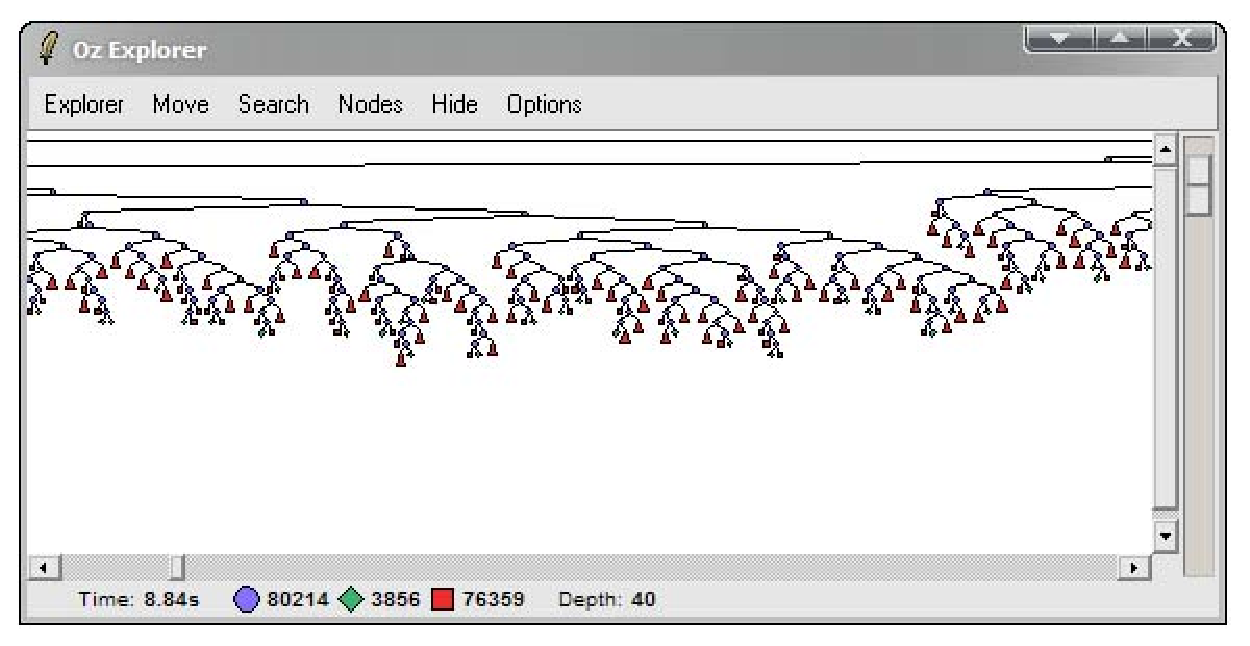
\includegraphics[width=0.6\textwidth]{../images/strasheela-search}
 \caption{Suche nach allen Lösungen von \textsl{All-Interval Series}, grüne
 Raute}
 \label{fig:strasheela-search}
\end{figure}


\section{MozEclipse}

Im Februar diesen Jahres startete Craig Ugoretz das Projekt 
\textsl{MozEclipse}\footnote{\url{http://gforge.info.ucl.ac.be/projects/mozeclipse/}}. 
Ziel dieses Projekts ist es, Mozart und Oz in die Eclipse IDE zu integrieren. 
Durch die Integration soll der Bekanntheitsgrad von Mozart/Oz steigen. Momentan 
ist Mozart in den Emacs integriert, der vor allem Anfängern einige 
Schwierigkeiten bereitet. Durch die Integration in Eclipse sollen die Hemmungen 
beseitigt werden, da viele Anwender gut mit Eclipse vertraut sind. Leider ist 
die Zukunft dieses Projekts noch sehr ungewiss, da es seit dem Anlegen der 
Projekt-Homepage keine weiteren Aktivitäten gab.